%\documentclass{acmsiggraph}                     % final
%\documentclass[annualconference]{acmsiggraph}  % final (annual conference)
%\documentclass[review]{acmsiggraph}            % review
\documentclass[widereview]{acmsiggraph}        % wide-spaced review
%\documentclass[preprint]{acmsiggraph}          % preprint

%% Uncomment one of the five lines above depending on where your paper is
%% in the conference process. ``review'' and ``widereview'' are for review
%% submission, ``preprint'' is for pre-publication, and ``final'' is for
%% the version to be printed. The ``final'' variant will accept the 
%% ``annualconference'' parameter, which changes the height of the space
%% left clear for the ACM copyright information.

%% The 'helvet' and 'times' packages define the typefaces used for
%% serif and sans serif type in this document. Computer Modern Roman 
%% is used for mathematics typesetting. The scale factor is set to .92
%% to bring the sans-serif type in line with the serif type.

\usepackage[scaled=.92]{helvet}
\usepackage{times}
\usepackage{latexsym}

%% The 'graphicx' package allows for the inclusion of EPS figures.

\usepackage{graphicx}

%% use this for zero \parindent and non-zero \parskip, intelligently.

\usepackage{parskip}

%% Optional: the 'caption' package provides a nicer-looking replacement
%% for the standard caption environment. With 'labelfont=bf,'textfont=it',
%% caption labels are bold and caption text is italic.

\usepackage[labelfont=bf,textfont=it]{caption}

%% If you are submitting a paper to the annual conference, please replace 
%% the value ``0'' below with the numeric value of your OnlineID. 
%% If you are not submitting this paper to the annual conference, 
%% you may safely leave it at ``0'' -- it will not be included in the output.

\usepackage{listings}
\usepackage{alltt}
\usepackage{subfigure}

%%\usepackage[caption=false]{subfig}

\onlineid{paper1041}

%% Paper title.

\title{Integration of X3D Geospatial in a Data Driven Web Application}

%% Author and Affiliation (single author).

%%\author{Roy G. Biv\thanks{e-mail: roy.g.biv@aol.com}\\Allied Widgets Research}

%% Author and Affiliation (multiple authors).


\author{Michael McCann\thanks{e-mail: mccann@mbari.org}\\MBARI
\and Byounghyun Yoo\thanks{e-mail: yoo@byoo.net}\\Korea Institute of Science and Technology
\and Don Brutzman\thanks{e-mail: brutzman@nps.edu}\\Naval Postgraduate School}


%% Keywords that describe your work.

\keywords{3-D Geography, X3D, geospatial, X3D-Earth, X3DOM, PostGIS, terrain rendering, sensor web, Oceanography, data visualization}

%%%%%% START OF THE PAPER %%%%%%

\begin{document}

\teaser{
\subfigure{
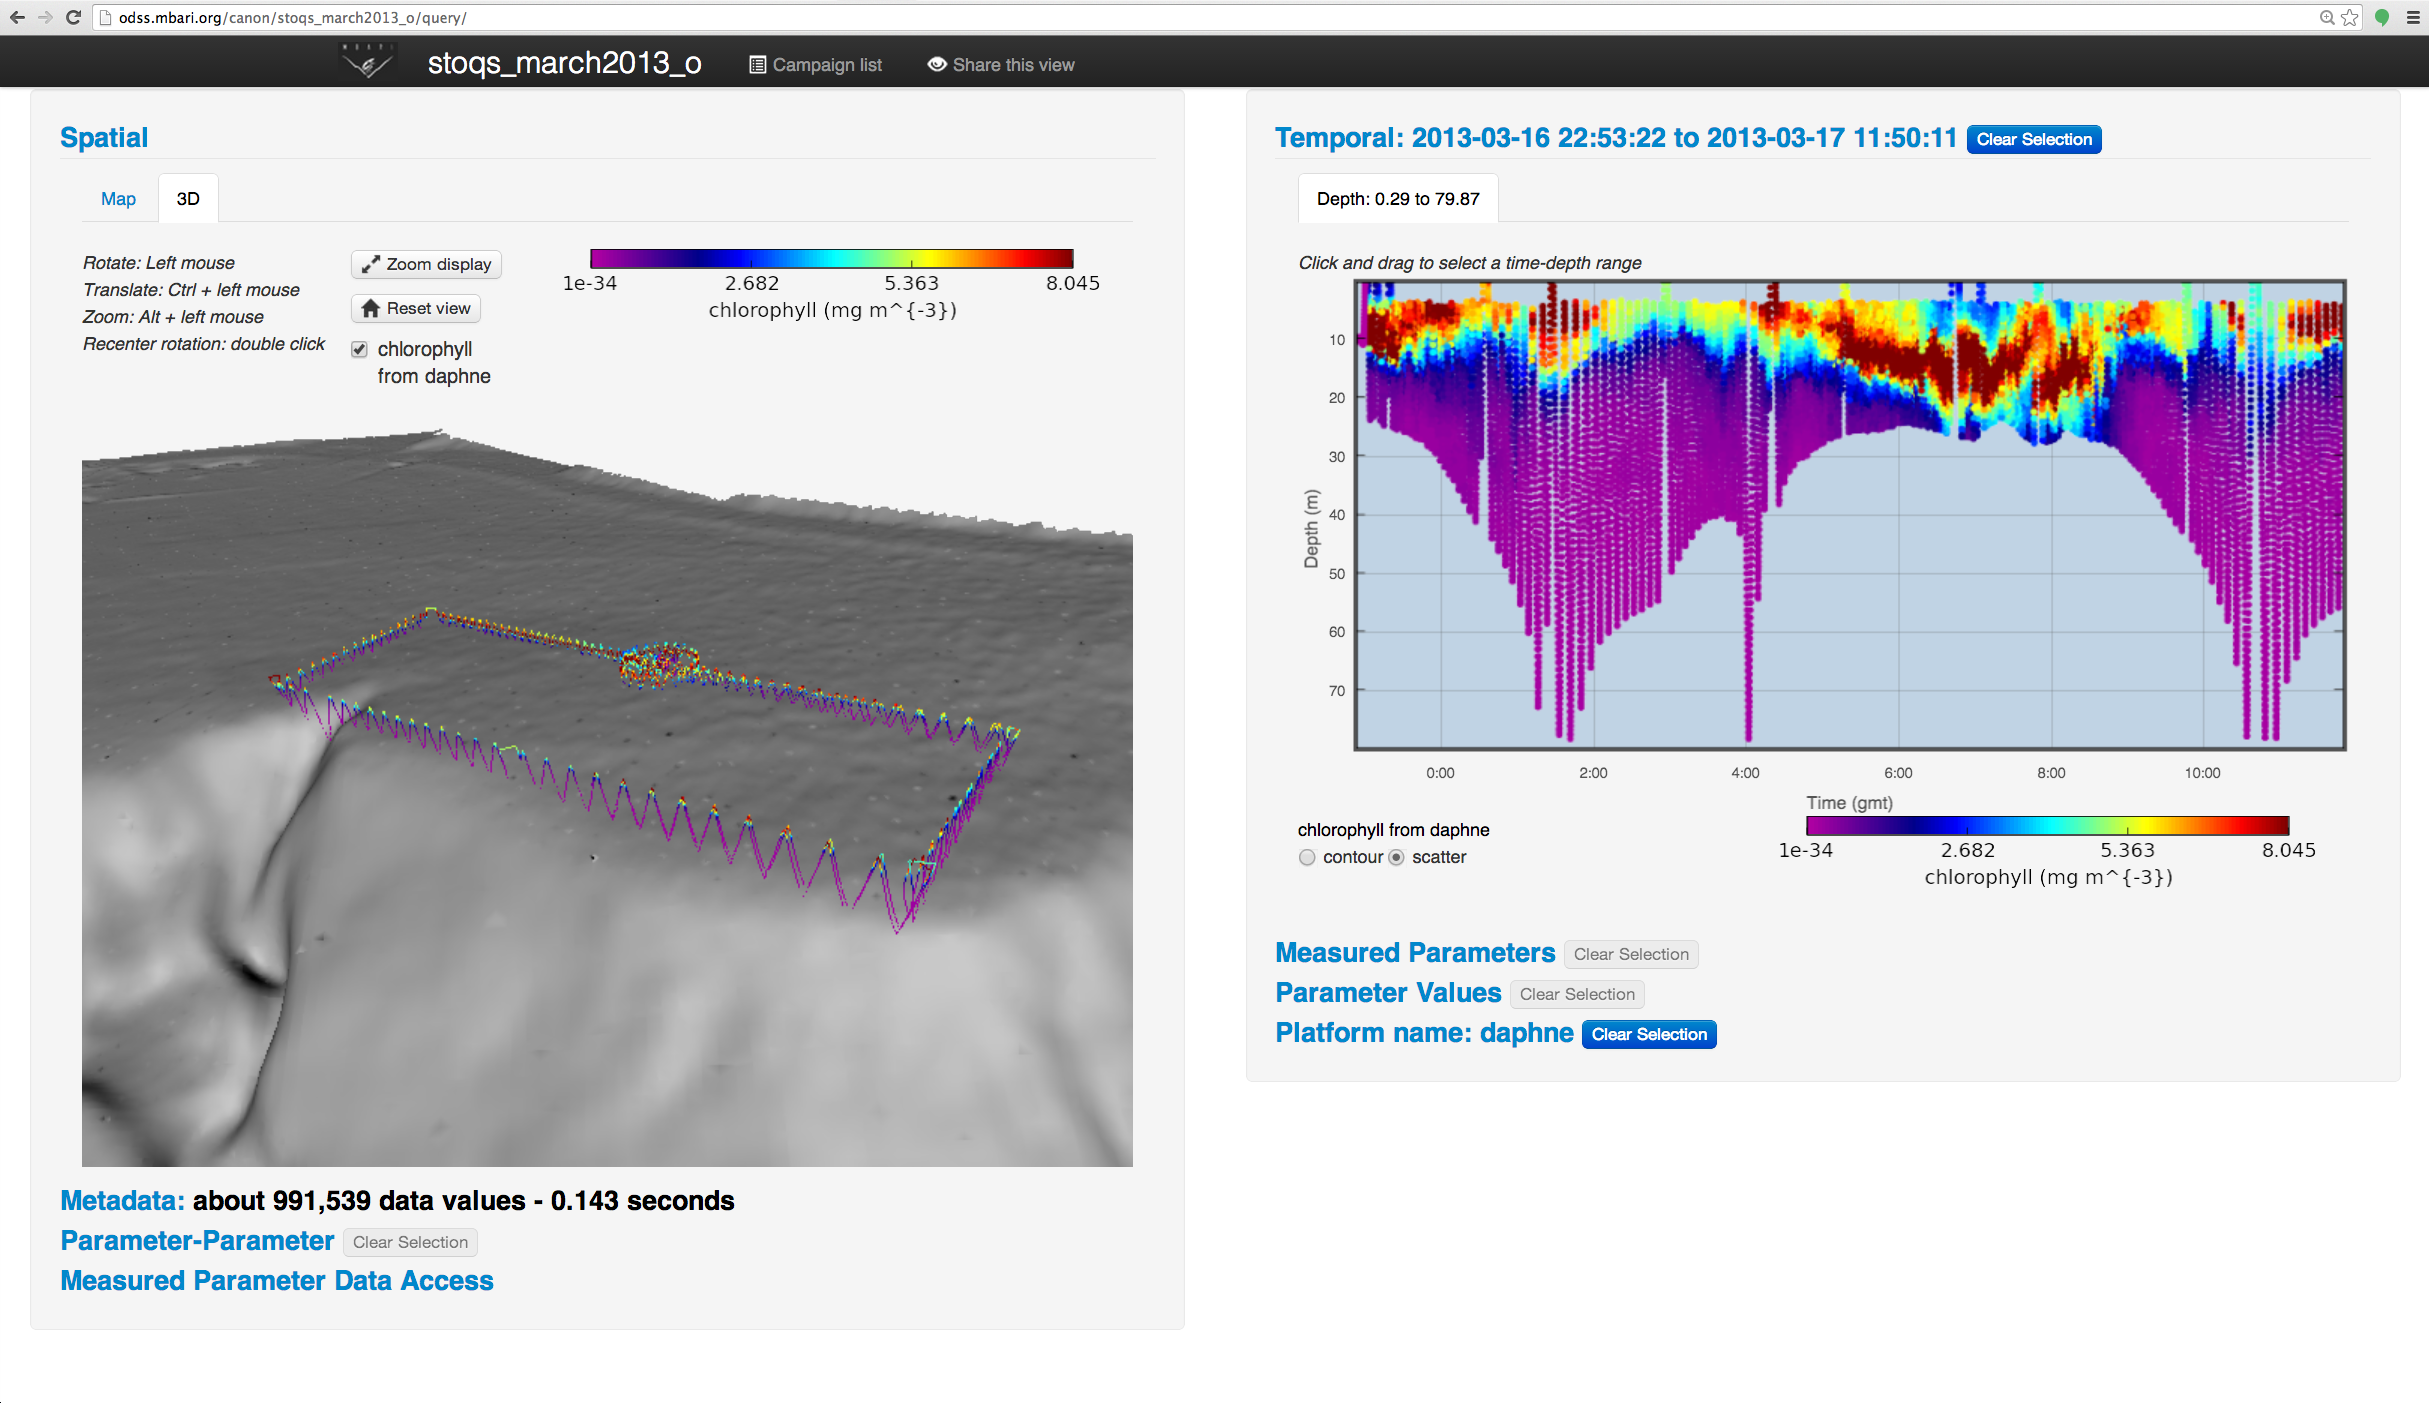
\includegraphics[width=7in]{STOQSUIscreencapture.png}

}

\caption{Screen capture of the STOQS web application showing underwater sensor data off the coast of southern California.}
\label{fig:STOQSscreencapture}
}




%% The ``\maketitle'' command must be the first command after the
%% ``\begin{document}'' command. It prepares and prints the title block.

\maketitle

%% Abstract section.

\begin{abstract}

Efficient analysis of growing types of oceanographic observations requires new approaches in data management and visualization. The Monterey Bay Aquarium Research Institute designed the Spatial Temporal Oceanographic Query System (STOQS) to create new capabilities for scientists to gain insight from their data. STOQS includes a web-based graphical user interface enabling effective data exploration across all dimensions of the data collection. This user interface is where X3D Geospatial has been integrated to enable 3D geospatial data visualization. This paper describes the STOQS User Interface, how X3DOM fits naturally within the framework, and discusses what service and content standards might be useful for sensor data portrayal. 


\end{abstract}

%% ACM Computing Review (CR) categories. 
%% See <http://www.acm.org/class/1998/> for details.
%% The ``\CRcat'' command takes four arguments.

\begin{CRcatlist}
\CRcat{I.3.7}{Computing Methodologies}{Computer Graphics}{Three-Dimensional Graphics and Realism}
\end{CRcatlist}

%% The ``\keywordlist'' command prints out the keywords.
\keywordlist

\section{Introduction}

%%\copyrightspace
%% The ``\copyrightspace'' command must be the first command after the 
%% start of the first section of the body of your paper. It ensures the
%% copyright space is left at the bottom of the first column on the first
%% page of your paper.

With increased ability to acquire measurements from oceanographic platforms such as ships, moorings, drifters, gliders and autonomous underwater vehicles (AUVs), the need to efficiently access and visualize the data they collect is growing. The Monterey Bay Aquarium Research Institute (MBARI) has designed and built the Spatial Temporal Oceanographic Query System (STOQS) specifically to address this issue \cite{imdis2013}. The fundamental issue of providing efficient management and access to multidisciplinary data is addressed by embracing existing standards and employing geospatial relational database technology along with modern web frameworks to build a tool that enables deep exploration of complex data sets. STOQS is an open source software project built upon a framework of free and open source software and is available for anyone to use and extend. For more information please see the STOQS code repository at http://code.google.com/p/stoqs.

Standards are important for the durability of data archived from oceanographic measurement programs. The data are unique and costly to collect. One of the standards used within the oceanographic community is NetCDF. It is a binary data format used commonly for gridded numerical model output and for remote sensing data. Because of its 20-plus year history of use, its flexibility, and because of its recent adoption as an Open Geospatial Consortium (OGC) standard, NetCDF is used for archiving of MBARI's \textit{in situ} measurement data.

The NetCDF data format (with the Climate and Forecast conventions) provide efficient data access for array data, such as from numerical models, because it provides indexed access to data on the coordinate dimensions. A NetCDF file performs like a mini database for data organized on a grid of longitude, latitude, depth, and time values. Retrieving spatial-temporal subsets from from an array happens with a direct seek into the NetCDF file. This is a the fastest way to retrieve data from a file on disk and is why NetCDF is popular for storing array-based data.

\begin{figure}[htbp]
\centering
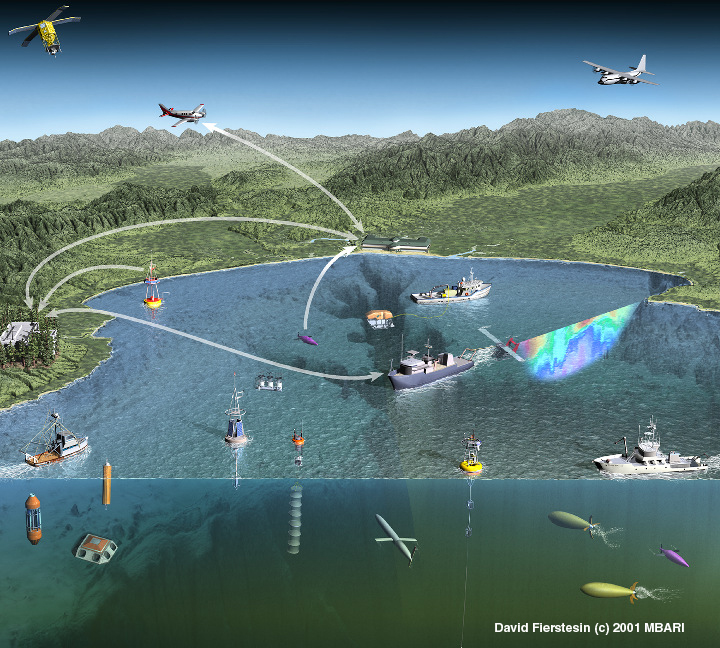
\includegraphics[width=3.3in]{MUSE_illus_pp.jpg}
\caption{Illustration of an oceanographic measurement campaign with multiple data collecting platforms.}
\label{fig:MUSE_illus_pp}
\end{figure}

This data access advantage does not exist for \textit{in situ} measurement data stored in NetCDF files. Trajectory data is increasingly being collected by a variety of new platforms. These include all the measurements taken by vehicles such as ships, drifters, gliders, and AUVs (Fig.~\ref{fig:MUSE_illus_pp}). These data are structured in NetCDF files with one coordinate dimension: time. Even though the data are distributed through space the only index into the mini-database NetCDF file is time. There is no efficient way to retrieve specific spatial-temporal data directly from a trajectory NetCDF file. For example, if an application program needed to extract just the surface temperatures from a glider data file --- where the glider samples the water column in a sawtooth pattern from 0 to 500 meters depth --- it would have to read all of the data from the NetCDF file and then perform the extraction. This is a very inefficient way to access data; if the trajectory data were in a fully indexed relational database then applications can have efficient data access. This is what STOQS provides. This paper describes its architecture and a web application that provides interactive 3D visualization using standard web technologies.



\section{STOQS}

STOQS has been in use at MBARI for over 3 years to help manage and visualize data collected during upper water column measurement campaigns where scientific goals center on improving our understanding of biological processes. The data consist primarily of measurements collected by moving platforms. The platforms have accurate clocks, Global Positioning Sensors and underwater inertial navigation sensors, and one or more instruments that measure parameters such as temperature, salinity, oxygen, nitrate, chlorophyll fluorescence, optical backscatter, and particle sizes. Some platforms can also capture water samples for later laboratory analysis. A typical workflow for is:
\begin{enumerate}
\item Install the STOQS software on a Linux server 
\item Vehicles conduct their missions, collecting data 
\item Create NetCDF files of the instrument data 
\item Construct and execute a STOQS load script
\item Access and visualize data using the STOQS UI
\end{enumerate}

\subsection{Architecture}

STOQS consists of a PostgreSQL/PostGIS database, Mapserver, and Python-Django running on a server and client-side technology (jQuery, OpenLayers, X3DOM, Twitter Bootstrap) running in a modern web browser (Fig.~\ref{fig:STOQSArch}) . The web application provides faceted search capabilities allowing a user to quickly drill into data of interest. Data selection can be constrained by spatial, temporal, and depth selections as well as by parameter values and platform names. The web application layer also provides a REST (Representational State Transfer) Application Programming Interface allowing tools such as Python, Matlab, and Google Earth to retrieve data directly from the database. The X3DOM JavaScript library provides interactive 3D views of the data in browsers that support WebGL.  

\begin{figure}[htbp]
\centering
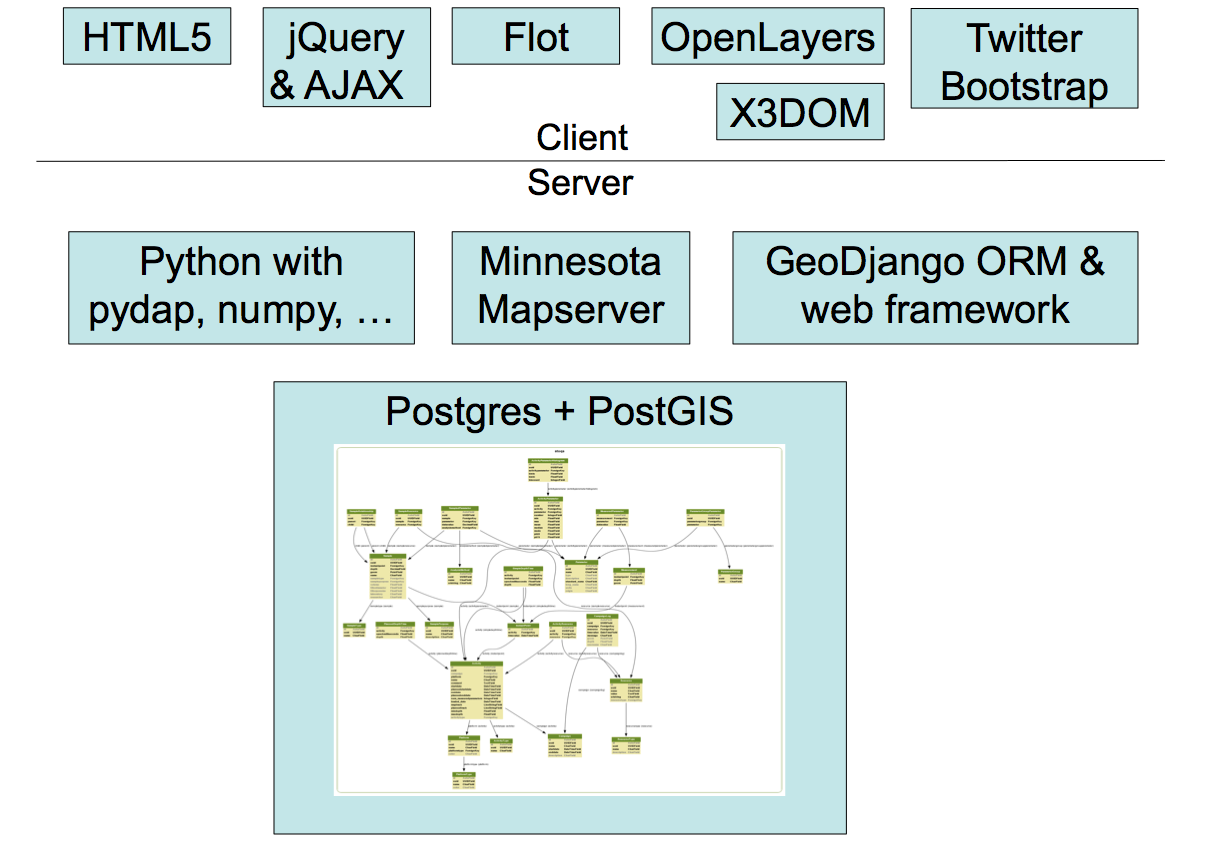
\includegraphics[width=3.3in]{STOQS_Architecture_withX3DOM.png}
\caption{Major software components that make up STOQS.}
\label{fig:STOQSArch}
\end{figure}

\subsection{STOQS User Interface}

The STOQS User Interface displays a map of the vehicle tracks and a time series of depth profiles of the vehicles (Fig.~\ref{fig:STOQSscreencapture}). The bold blue letter text items are each sections that may be expanded revealing lists of items that may be selected for filtering, data selection, and plotting. If a platform is selected for filtering then only the information from that platform are shown in the other sections of the interface. Any selection initiates an instant update of the other items that may be selected. With this faceted search capability the user can quickly narrow a selection for data of interest. For instance in Fig.~\ref{fig:STOQSscreencapture} the platform "daphne"  and a time range of about a half a day have been selected. The interface is reactive to browser screen size and behaves appropriately when viewed on tablets and smart phones.

Within the web application data are retrieved directly from the database via XHR (XMLHttpRequest) requests delivering data in JSON (JavaScript Object Notation) data structures. Client-side JavaScript code then formats these data as needed for display in the web page. Any DOM (Document Model Object) element, such as buttons and checkbox labels can be updated with data from the database. In fact, requested data can update any DOM element, including elements in the 2D Temporal Flot plot an in  X3D scene graphs placed anywhere in the web page. 

The overall design approach follows the so-called Shneiderman's mantra: "Overview first, zoom and filter, then details-on-demand" \cite{Whitney:2012:DIN:2597850}. This is in contrast to other data portal web sites which often present the user with empty text boxes in which unfamiliar users are at a loss on what to enter. The STOQS UI adheres to about 9 of the 12 elements of interactive dynamics described in \cite{Heer:2012:IDV:2133416.2146416}.


\section{Geospatial}

\subsection{2D Map Display}
The default spatial view in the STOQS UI is a 2D OpenLayers generated map. It shows simplified tracks of the vehicles over the selected basemap. The ESRI Ocean basemap is the default, but users can also select Open Street Maps and GEBCO \& NOAA Tiles, which is a local tile set for use aboard research vessels that do not have Internet connectivity. The track lines are generated on the server with a dynamically generated mapserver configuration file. Mapserver queries the database and builds image tiles which are then transmitted to the client using the OGC Web Map Service (WMS) protocol. As some campaigns contain dozens of tracks this approach performs better than individual transmission of vector data to the OpenLayers client code. Because WMS is a well established standard the server and client components - developed by different organizations - are able to work together using agreed upon request and response messages. If a user selects a Measured Parameter for plotting then a checkbox appears under the map for presentation of the sensor data as colored tracks on the map. These data are retrieved from the server with an XHR request and then delivered to OpenLayers as a vector layer in KML format. Performance degrades with more than about 300 points therefore server-side code subsamples large responses in order to maintain application responsiveness. 

\subsection{3D and DOM Updates}

Next to the Map tab in the Spatial section is a 3D tab. This 3D tab appears only for databases in which a terrain model has been loaded. A Python dictionary specifies the needed parameters for the STOQS UI to display a 3D terrain "basemap" (Fig.~\ref{fig:x3dTerrains}). Logic in the client code maps the position, orientation, and centerOfRotation values to the corresponding DOM elements in the scene graph. (The next section describes ways to construct X3D terrain models.)

\begin{figure}[htbp]
\centering
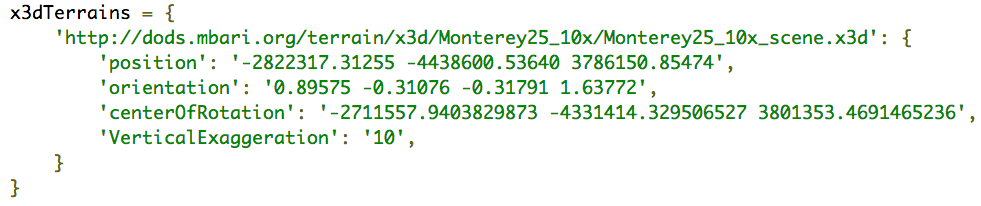
\includegraphics[width=3.3in]{x3dTerrains.png}
\caption{Dictionary of terrain information loaded into STOQS.}
\label{fig:x3dTerrains}
\end{figure}

Selected Measured Parameter data are delivered to the Spatial 3D display when a radio button and the checkbox is checked. The process for the update of the display is:

\begin{enumerate}
\item HTML contains X3D scene graph elements for the web page: Fig.~\ref{fig:Spatial3D_DOM}
\item Data are received by the browser from an XHR request in JSON format: Fig.~\ref{fig:JSONData}
\item jQuery JavaScript code takes the values from the JSON and writes them to the scene graph elements: Fig.~\ref{fig:jQueryDOMUpdate}
\end{enumerate}

\begin{figure}[!htbp]
\centering
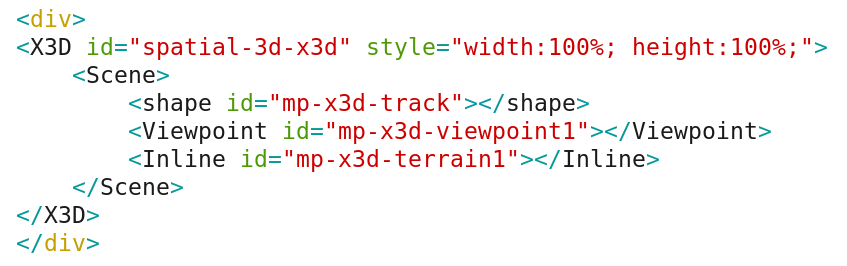
\includegraphics[width=3.3in]{Spatial3D_DOM.png}
\caption{X3D scene graph within the HTML before being updated.}
\label{fig:Spatial3D_DOM}
\end{figure}

\begin{figure}[!htbp]
\centering
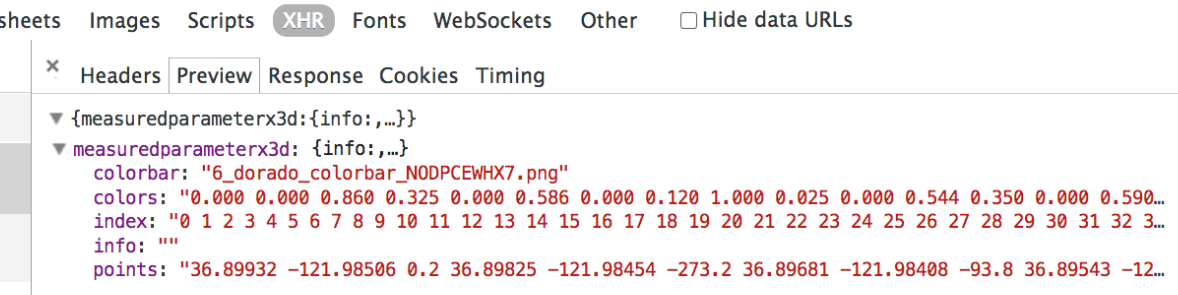
\includegraphics[width=3.3in]{JSONData.png}
\caption{Measured Parameter X3D data in JSON format returned by XHR request.}
\label{fig:JSONData}
\end{figure}

\begin{figure}[!htbp]
\centering
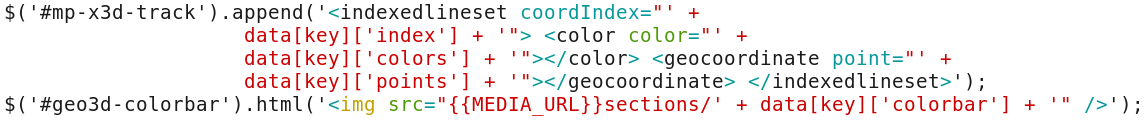
\includegraphics[width=3.3in]{jQueryDOMUpdate.png}
\caption{JQuery JavaScript code that updates the X3D DOM elements.}
\label{fig:jQueryDOMUpdate}
\end{figure}

Updates are triggered by any selections in the UI that would result in different data being displayed. An example would be selecting a smaller depth-time region in the Temporal section. Sensor data are represented in X3D as an IndexedLineSet built out of geocoordinate points, which is this case are latitude, longitude, and depth relative to the WGS84 ellipsoid, the default geosystem. X3D Geospatial performs the conversion of geodetic coordinates to geocentric coordinates which is the native coordinate system used by X3D Geospatial.

\section{Terrain Rendering}

\subsection{GeoElevationGrid}

As explored by \cite{yoo09} the Earth's terrain can be represented using GeoElevationGrid nodes. High resolution terrain can be structured in a nested quad-tree tile set using GeoLOD nodes. For representing data for the entire globe a multi-resolution approach such as this is a common. In fact, popular globe viewers such as Google Earth use this approach with sophisticated techniques to decide which tiles to load and unload depending on the users viewpoint and motion through the world. These techniques improve performance, are often proprietary, and can help distinguish a product within the marketplace. Similar techniques have not yet found their way into open source implementations of X3D Geospatial. However, small regions of the Earth can be represented in a single tile with enough horizontal resolution to be useful. MBARI's oceanographic campaigns are typically constrained to small geographic regions such as Monterey Bay and San Pedro Bay. For these regions a 50 meter gridded terrain model represented as a single GeoElevationGrid has less than a million vertices, which is effectively  rendered by today's 3D graphics hardware.  

\subsection{POP Geometry}

In 2013 \cite{Limper:2013:FDW:2466533.2466536} introduced Progressively Ordered Primitive (POP) buffers in X3DOM. Large POP geometry meshes (up to 1.5 million faces) are rendered with very good performance on today's computers with X3DOM. Advantages of representing bathymetric data in meshes is addressed by \cite{Becker:2005:NPN:1650409.1650513}. Meshes, in contrast to regular grids, are able to use fewer larger triangles for flat and smooth portions of terrain and more smaller triangles for the rugged portions of terrain. Besides providing more accurate representations of bathymetry meshes can also represent overhangs and caves, whereas GeoElevationGrids cannot. The workflow for creating the x3dterrain files using open source tools GMT \cite{GMT} and Meshlab \cite{Meshlab} is similar to that used in \cite{Silvestre}:

\begin{itemize}
\item Use GMT to create a point cloud in geocentric coordinates with 10x vertical exaggeration:
\begin{verbatim}
gmt grd2xyz Monterey25.grd \
  --D_FORMAT=%f | sed '/NaN/d' | \
  awk '{print $1, $2, 10 * $3}' | \ 
  mapproject -E --D_FORMAT=%f > \
  Monterey25_10x.asc
\end{verbatim}
\item Process interactively in Meslab:
\begin{itemize}
\item Load .asc file
\item Fliter - Point Sets - Compute normals for point sets
\item Filter - Surface Reconstruction: Poisson (Octree Depth: 12, Solver Divide: 10)
\item Filter - Remeshing, Simplification and Reconstruction - Quadric Edge Collapse Decimation:
\begin{itemize}
\item Target number of faces: 1,500,000 
\item Preserve Normal
\item Preseve Topology
\item Optimal Position of Simplified Vertices
\item Planar Simplification
\item Post-simplification cleaning
\end{itemize}
\item Cleanup (with plenty of intermediate saves)
\item Filter - Smoothing� - Laplacian smooth (surface preserve)
\item Export mesh to .ply
\end{itemize}
\item Build X3D files with InstantReality aopt tool:
\begin{verbatim}
aopt -i Monterey25_10x-smooth.ply \
  -F Scene -b Monterey25_10x-opt.x3db
aopt -i Monterey25_10x-opt.x3db \
  -f PrimitiveSet:creaseAngle:4 -V \
  -K "binGeo/:ib" -N Monterey25_10x.html
\end{verbatim}
\end{itemize}

These operations result in a static web page where the results can be tested for fidelity and performance. In order for the terrain model to be included in the STOQS UI the Scene elements are extracted from the HTML into a separate scene X3D file. This file and the associated binGeo files are what is referenced in Fig.~\ref{fig:x3dTerrains} for loading into STOQS. Fig.~\ref{fig:Monterey25_lrauvs} shows the terrain built with the above steps along with a the chlorophyll measurements of month-long deployments of 2 AUVs in Monterey Bay.

\begin{figure}[htbp]
\centering
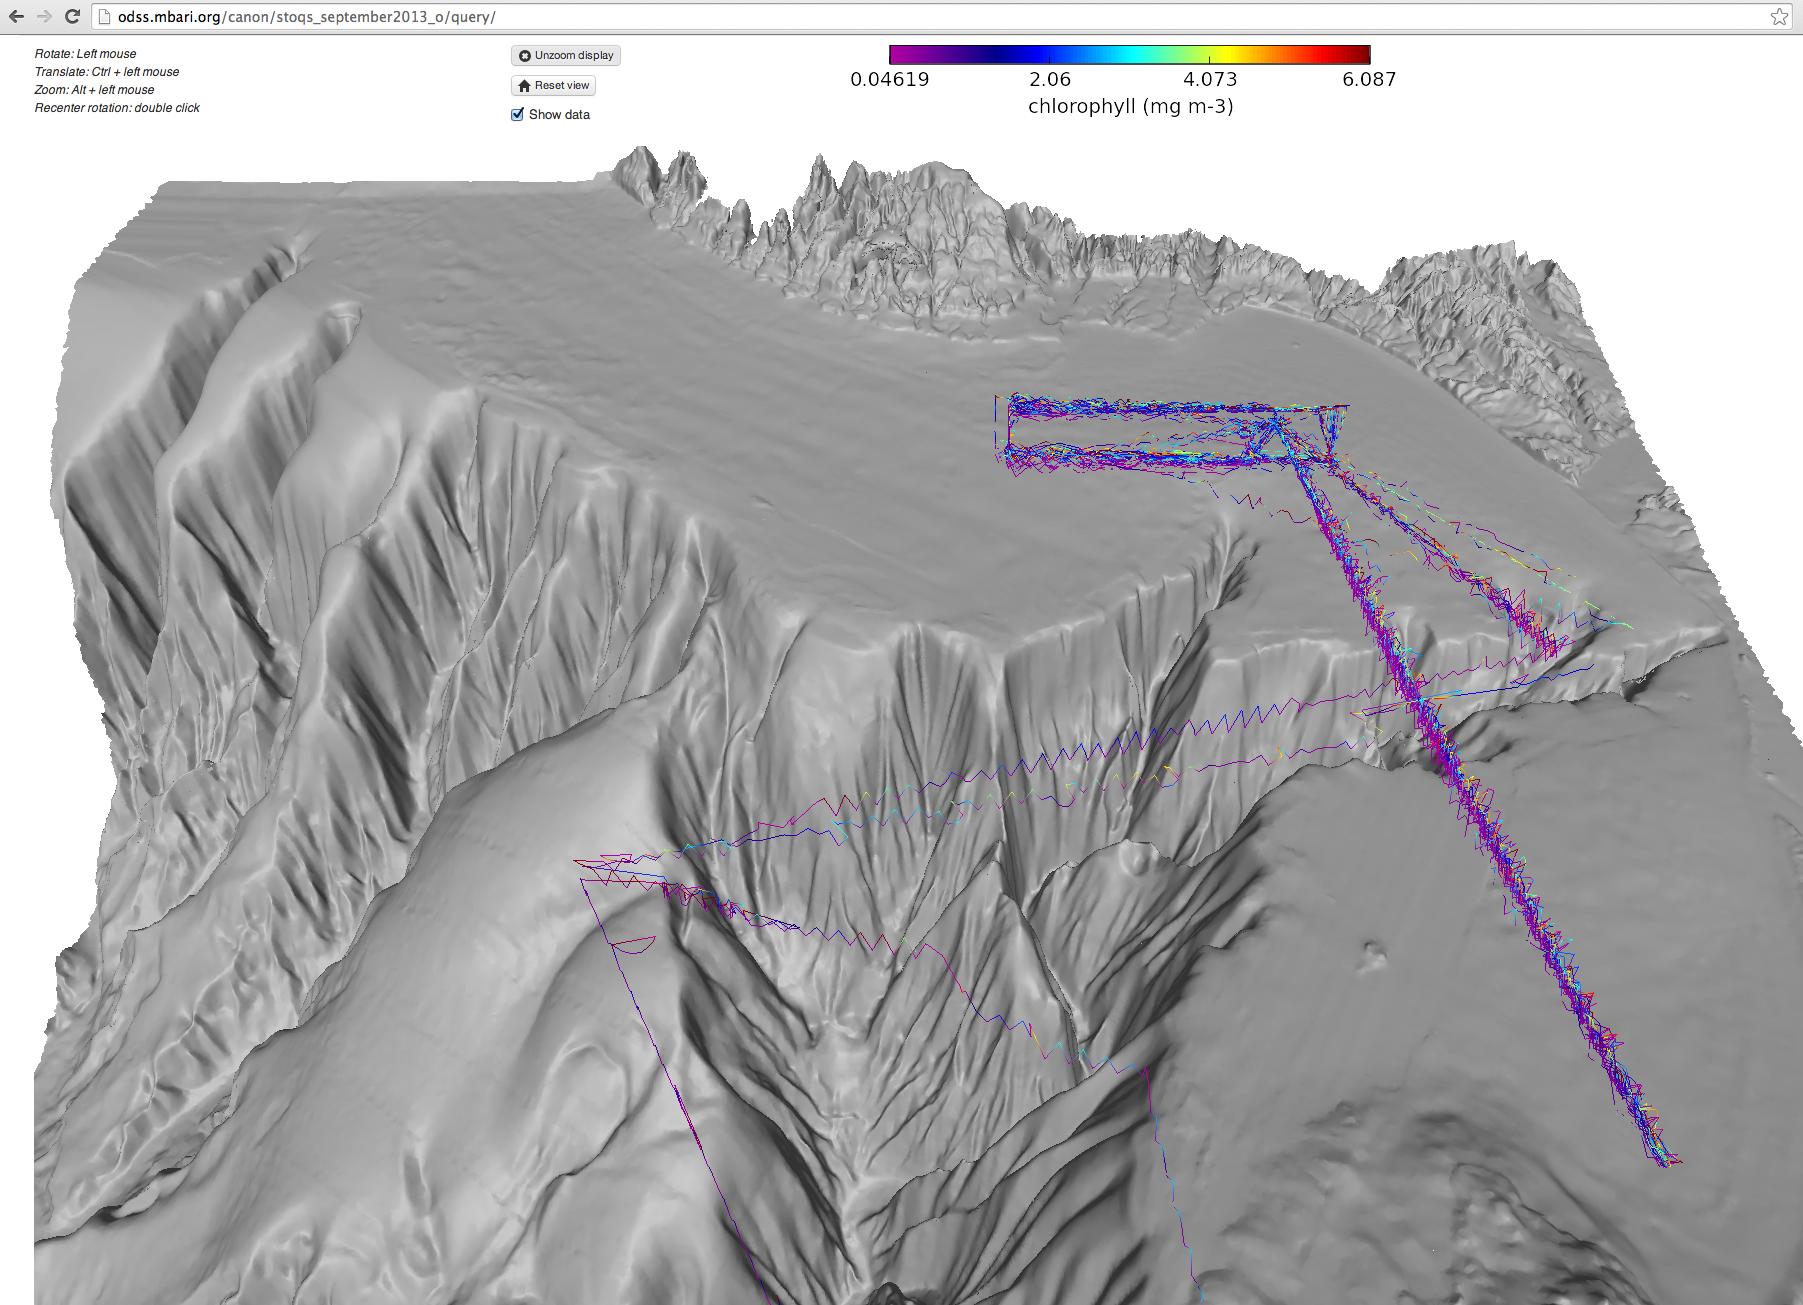
\includegraphics[width=3.3in]{Monterey25_lrauvs.png}
\caption{POP Geometry of 25m resolution Monterey Bay terrain with AUV measured chlorophyll data rendered by X3DOM in STOQS.}
\label{fig:Monterey25_lrauvs}
\end{figure}


% Prevent hyphenation


\section{Discussion}
The content standard of X3D together with modern web technologies gives a skilled developer quite a bit of flexibility and capability to build data rich 3D scenes. Comparing the Map display of data with the 3D display in the STOQS UI is useful for considering what protocol standards may be useful for 3D data. The Map display receives data via the OGC's Web Mab Service (WMS) protocol. Is there an equivalent protocol for 3D data? Do we need one? For the first question the OGC 3D Portrayal Interoperability Experiment (3DPIE) \cite{3DPIE} proposed best practices to use within the city modeling domain.  For medium and thick clients (those able to render interactive 3D scenes) a GetScene request will return an entire X3D scene in whatever coordinates the server generates. WIth this architecture the server can guarantee consistency of all the elements within a scene. A disadvantage is that all content in the scene must come from the same server which determines independently what 3D coordinate reference system is used.

With the 2D display content is able to be received and "mashed up" from multiple servers. The basemap is provided by the ESRI or Open Street Map servers and the measurements from the platforms are provided by the STOQS server. The WMS protocol enables this, mainly through its requirement that each GetMap request include a CRS field specifying the EPSG code for the coordinate reference system of the map.

There are several use cases for 3D mashup capability. The 3DPIE identified sensor data as a source for portrayal but left the implementation of a sensor service capability for a future effort. Data representing such things as atmospheric pollutants could be retrieved from external servers and could be portrayed as a transparent cloud within a model of a city. Examples within the oceanographic domain include adding remotely sensed surface chlorophyll fluorescence data to the scene from servers at NASA and inclusion of features from numerical ocean circulation models. 

The STOQS platform is an ideal environment for experimenting with various ways to portray data and understand the patterns of data access that lead to best practices and eventually internationally agreed upon standards. Future work for the project includes: 1) giving the user the option of presenting measurement data as a PointSet instead of an IndexedLineSet, 2) improving X3DOM's implementation of the Geospatial component, and 3) testing the mashup of data from external servers.


\section{Conclusion}

Initial experiments with integrating X3D with a data driven web application have proven quite successful. The capability that X3DOM provides for updating scene graph elements with data from a database opens many possibilities for visualizing sensor data within the context of other 3D geospatial content. 


\section*{Acknowledgements}

Appreciation is given to the numerous people involved in the deployment, recovery, operation and data handling for all of the platforms whose data are presented here. Development of STOQS is supported by the David and Lucile Packard Foundation at the Monterey Bay Aquarium Research Institute. It was inspired by the MOQuA tool originally developed by Mike Godin \cite{godin05}. 




\bibliographystyle{acmsiggraph}
\nocite{*}
\bibliography{IntegrationOfX3DGeospatial}




\end{document}
